
% TODO
Halllowoeo dsff dfs  df dss f \cite{Carrier.06.01.2022}  welt1


hallo

Hallo \cite{Sciencedirect.07.01.2022}  welt




Struktur EINFACH GENAU SO!!!!!!

\textbf{1. Technischer Hintergrund\\}

Beschreiben Sie in diesem Abschnitt die technische Funktionsweise des EXT3 Dateisystems. 


bissl history... bissl blocl, etc siehe weiter unten!\\


Gehen Sie dabei im speziellen auf die folgenden Fragestellungen ein:\\

a) Wie speichert das Dateisystem Daten (Inhaltsdaten)?\\

b) Wie speichert das Dateisystem Metadaten (Dateinamen, Größe, Berechtigungen, Zeitstempel, ...)?\\

c) Was passiert bei einem EXT3 Dateisystem im Hintergrund, wenn eine Datei erzeugt wird?\\

d) Was passiert bei einem EXT3 Dateisystem im Hintergrund, wenn eine Datei gelöscht wird?\\

Generieren Sie für die Bearbeitung ein eigenständiges kleines „praktisches“ Beispiel, an dem Sie den technischen Hintergrund anschaulich erläutern.\\


\textbf{2. Forensische Analyse\\}

Beschreiben Sie in diesem Abschnitt forensischen Konzepte zur Analyse eines EXT3 Dateisystems.\\
Gehen Sie dabei im speziellen auf die folgenden Fragestellungen ein:\\

a) Welche forensischen Konzepte existieren für die Auswertung eines EXT3 Dateisystems?\\

b) Welche Ansätze unter EXT3 gibt es, um eine gelöschte Datei wiederherzustellen?\\

Demonstrieren Sie insbesondere Aufgabenstellung 2b) anhand Ihres kleinen „praktischen“ Beispiels aus Aufgabenstellung 1.\\










\section{Geschichte des EXT Dateisystems}

Das sogenannte \ac{ext} war das erste einer Reihe von Dateisystemen welches speziell für Linux entwickelt wurde und damals das minix Dateisystem ablöste. EXT in Version 1 ist mittlerweile allerdings veraltet und wird in aktuellen Linuxdistributionen nicht mehr verwendet. Die folgenden Erweiterungen existieren:

\begin{itemize}
	\item ext2 - Führte separate Zeitstempel für Dateizugriffe, inode- und Datenmodifikation. Bringt keine Unterstützung für journaling.
	\item ext3 - Führt journaling ein (und ist required!)
	\item ext4 - Unterstützung für fast fsck[1], native filesystem encryption[2], journaling, jedoch auch für non-journaling.
\end{itemize}

% TODO
- Einfach das ext2 pdf lesen (ext3 ist einfach ext2 MIT JOURNALING!!!)
- Journaling beschreiben! -> bedeutet das DS hat einen extra Bereich in dem ALLE Änderungen getrackt werden. Im Falle eines Systemcrash kann somit die Wahrscheinlichkit von FS corruption verringert werden (!?!?!??!)
- memory faster than writes to disk
- 

- Intro to EXT allgemein, siehe Fragen in der Aufgabenstellung


\section{Technische Hintergründe zum EXT3 Dateisystem}

EINFACH HIER ERSTMAL DIE *DEFINITIONS* DURCH!!!!!!!!!!!
https://raw.githubusercontent.com/skeledrew/ext4-raw-reader/master/ext2.pdf

Creating filesystem with 7680000 4k blocks and 1921360 inodes

==> wir haben also immer 4k BLOCKS!!! mit N inodes!!!!!!!!!!

Writing inode tables:  48/235
WAS SIND inode TABLES!!?!??!?!?!?! 1921360 inodes in 235 tables?!?! NOPE. 235 Block Groups - SEE meine Zeichnung auf Schmierzettel!
1921360 / 235
8176 inodes per BLOCK GROUP
\\


a) Wie speichert das Dateisystem Daten (Inhaltsdaten)? 

ZeichnungEN schmierzettel und mehr! hier nochmal paar Zeichnungen schön hübsch rein, CONTENT!

b) Wie speichert das Dateisystem Metadaten (Dateinamen, Größe, Berechtigungen, Zeitstempel, ...)? 

INODE ERKLÄREN!!!\\
\\

sudo istat -o 0 -r /dev/sdb 24530
inode: 24530
Not Allocated
Group: 3
Generation Id: 2609919107
uid / gid: 1000 / 1000
mode: rrw-rw-r--
size: 0
num of links: 0

Inode Times:
Accessed:	2022-01-07 15:35:26 (CET)
File Modified:	2022-01-08 13:01:30 (CET)
Inode Modified:	2022-01-08 13:01:30 (CET)
Deleted:	2022-01-08 13:01:30 (CET)

Direct Blocks:
Staring address: X, length: 1  Sparse



c) Was passiert bei einem EXT3 Dateisystem im Hintergrund, wenn eine Datei erzeugt wird?  

TODO: file und dir vergleichen!

d) Was passiert bei einem EXT3 Dateisystem im Hintergrund, wenn eine Datei gelöscht wird?

TODO: file und dir vergleichen!

rm -rf file -> "nullt" die inode die auf diese datei oder dir zeigt, der BLOCK jedoch ist immer noch auf der platte und kann betrachtet werden! DATEN ALSO NOCH DA! nur inodes werden genullt!
IM FALLE EINES DIR: 
alle dateien werden dann halt "unlinked" von diesem dir. die haben vermutlich dann noch ihre inodes, aber der link zum dir fehlt halt !??!?!?



\subsection{Praktisches Beispiel}

Daten erstellen und Löschen - siehe Aufgabenstellung!

\section{Forensische Analyse des EXT3 Dateisystems}

a) Welche forensischen Konzepte existieren für die Auswertung eines EXT3 Dateisystems? 

TODO: ZUERST sleuthkit Vorstellung


sudo fsstat -o 0 /dev/sdb
FILE SYSTEM INFORMATION
--------------------------------------------
File System Type: Ext3
usw... CHECK DAS GENAU!


b) Welche Ansätze unter EXT3 gibt es, um eine gelöschte Datei wiederherzustellen?

vorher ggf mal ls -li und inode number merken!
dann rm -rf hier zeigen

UND dann SLEUTHKIT
Rekursives Anzeigen aller Dateien, inklusive gelöschter Dateien:
sudo fls -o 0 -r /dev/sdb
...
r/r * 24530:	Bildschirmfoto vom 2022-01-07 11-59-24.png

Dann Wiederherstellen der Datei mit inode 24530 mittels icat:
sudo icat -o 0 /dev/sdb 24530 > image.jpg


TODO: THIS WORKED!!!!!!!! auch mit rm -rf! MEHR EXPERIMENTE. WIE FUNZT DAS?
irgendwie mit dem journal. read man!
sudo ext4magic /dev/sdc -M




TODO: autopsy vorstellung und BEISPIEL!!!!!!!!!!!!!!!!!!!!!!!????????????

TODO recover on linux:\\
	https://possiblelossofprecision.net/?p=1216\\
	weitere tools linux: foremost, dff? ...\\
		-> https://www.cgsecurity.org/wiki/PhotoRec
	sudo ext4magic /dev/sdc -M

TODO:
READ this: https://en.wikipedia.org/wiki/Ext3




\subsection{Praktisches Beispiel}

1. Files erstellen und dann löschen (1mal mit papierkorb 1mal mit rm -rf - ggf auch ganzes DIR!)
2. Forensische Arbeitskopie erstellen:

\begin{lstlisting}
$ sudo dd if=/dev/sdc of=usb.dd bs=512 conv=noerror,sync status=progress
\end{lstlisting}

commands format stick:

lsblk to find mounted devices
unmount device:  sudo umount /dev/sdc1

hier RICHTIG SCHÖN ZEIT LASSEN, IMMER NEUE ZEILE MIT KÄSTCHEN!!!!!

sudo mkfs -t ext3 /dev/sdc
\begin{figure}[H]
	\centering
	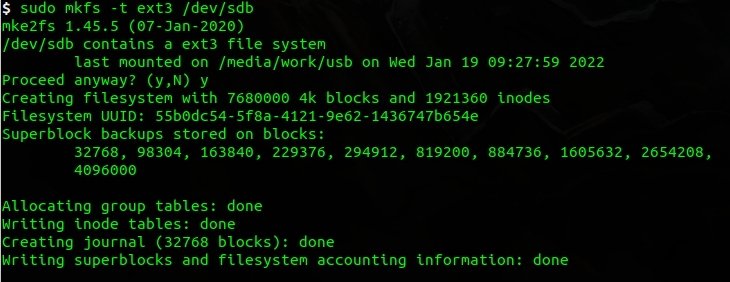
\includegraphics[width=12cm,keepaspectratio=true]{pictures/createfs.png}
	\caption{
		Erstellen eines EXT3 Dateisystems auf einem USB Stick
	}
	\label{fig:createfs}
\end{figure}
TODO: GENAU BESCHREIBEN WAS DA PASSIERT!



Datei erstellen, löschen ist ja bereits in TEIL1 passiert! darauf verweisen, daran werde ich nun weiterarbeiten hier!

ERSTMAL ARBEITSKOPIE!!! ganzen prozess erklären (siehe forensics BOOK -> why, how etc...)
schön mit screenshots und code ausschnitten!
